% questions.tex —— 1985 年·广东卷·理工农医类 · 题目内容片段（无答案）
% 由 tools/generate_projects.py 依来源总账自 1985/1985_数学真题_广东理工农医类_试题.md 生成，勿手改（改源 MD 后重跑）


\begin{gktip}
按固定来源 PDF 转录。原 PDF 未见纸面页码。题头数字是唯一内部顺序，HTML 注释保存原卷在卷/大题内重新起算的显示题号；疑字以 U 编号保留。
\end{gktip}

\gkpart{第一卷 一、填空与画图（20 分）}

本题共 10 小题，每小题 2 分；1–9 填空，10 画图。

\begin{question}
\gkti{1}函数 $y=\sqrt{\operatorname{arctg}(1-x)}$ 的定义域是＿＿。

\end{question}
\begin{question}
\gkti{2}如果 $f(1/x)=\dfrac{x}{1-x^2}$，则 $f(x)=$＿＿。

\end{question}
\begin{question}
\gkti{3}如果一个圆锥底面的半径增大到原来的三倍，但要保持它的体积不变，则其高必须缩小到原来的＿＿。

\end{question}
\begin{question}
\gkti{4}在直角坐标系中，通过点 $(0,0)$、$(1,0)$ 和 $(0,2)$ 的圆的方程是＿＿。

\end{question}
\begin{question}
\gkti{5}$\operatorname{tg}\dfrac\pi5+\operatorname{tg}\dfrac{2\pi}5+\operatorname{tg}\dfrac{3\pi}5+\operatorname{tg}\dfrac{4\pi}5$ 的值等于＿＿。

\end{question}
\begin{question}
\gkti{6}$\displaystyle\lim_{n\to\infty}\frac{1+4+7+\cdots +(3n-2)}{n(n+1)}$ 的值等于＿＿。

\end{question}
\begin{question}
\gkti{7}函数 $y=\sin^2(2x)$ 的最小正周期是＿＿。

\end{question}
\begin{question}
\gkti{8}已知函数 $f(x)=ax^5+\operatorname{arctg}x$，其中 $a$ 为常数，且 $f(2)=10$，则 $f(-2)$ 的值是＿＿。

\end{question}
\begin{question}
\gkti{9}已知圆的方程为 $x^2+(y-2)^2=9$，用平行于 $x$ 轴的直径把圆分为上下半圆，则以上半圆弧（包括端点）为图象的函数表达式是＿＿。

\Needspace{0.4\textheight}
\end{question}
\begin{question}
\gkti{10}请把方程 $y\sqrt{x}-y-2x+2\sqrt{x}=0$ 所表示的曲线画在右边的直角坐标系中。
\nopagebreak[4]
\begin{center}% 1985 广东理工农医类第一卷一（10）：题面提供给考生作图的空白坐标系。
\begin{tikzpicture}[scale=0.8,>=stealth]
  \draw[->,thick] (-0.4,0)--(5.4,0) node[right] {$x$};
  \draw[->,thick] (0,-1.2)--(0,3.8) node[above] {$y$};
  \fill (0,0) circle (1.1pt) node[below left] {$O$};
  \foreach \x in {1,2,3,4,5} {
    \draw (\x,0.07)--(\x,-0.07);
  }
  \foreach \y in {-1,1,2,3} {
    \draw (0.07,\y)--(-0.07,\y);
  }
  \node[below] at (1,-0.12) {$1$};
  \node[left] at (-0.12,1) {$1$};
\end{tikzpicture}
\end{center}
\nopagebreak[4]
\end{question}
\gkpart{第一卷 二、单项选择}

共 20 小题；1–16 每题 2 分，17–20 每题 3 分。每题 A–E 五个结论中只有一个正确；不选、选错或选出超过一个，得 0 分。原题提到把代号写在“下表”，但固定 PDF 题面页未见相应答题表（U1）。

\Needspace{0.4\textheight}
\begin{question}
\gktiwithlabel{11}{1}函数 $y=2^{-x}$ 的图象的大致形状是（ ）。A–E 为五幅坐标图：A 递增且过 $(0,1)$；B 递减且标 $(1,1)$；C 递减并穿过 $(1,0)$；D 递增并穿过 $(1,0)$；E 递减且过 $(0,1)$。
\nopagebreak[4]
\begin{center}% 1985 广东理工农医类第一卷二（1）：原卷 A–E 五个函数图示，曲线只表达形状。
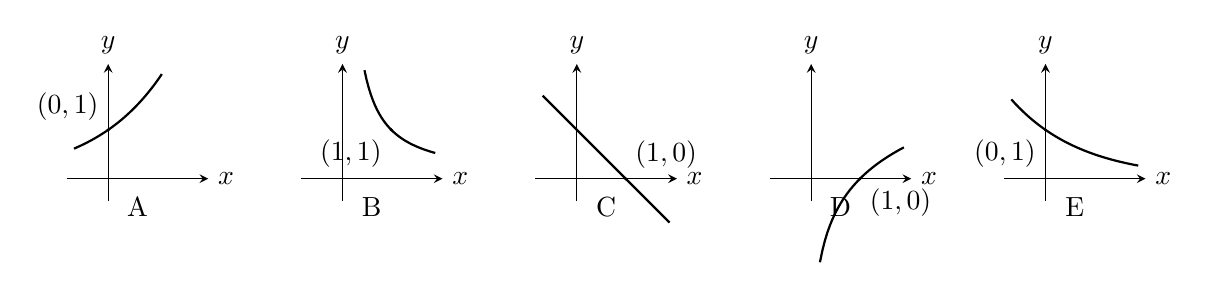
\begin{tikzpicture}[scale=0.62,>=stealth]
  \foreach \x/\label in {0/A,4.8/B,9.6/C,14.4/D,19.2/E} {
    \begin{scope}[shift={(\x,0)}]
      \draw[->] (-0.85,0)--(2.05,0) node[right] {$x$};
      \draw[->] (0,-0.45)--(0,2.35) node[above] {$y$};
      \node at (0.6,-0.58) {\label};
    \end{scope}
  }
  % A 递增，过 (0,1)
  \begin{scope}
    \draw[thick,domain=-0.7:1.1,samples=35] plot (\x,{2^\x});
    \fill (0,1) circle (1pt) node[above left] {$(0,1)$};
  \end{scope}
  % B 递减，标 (1,1)
  \begin{scope}[shift={(4.8,0)}]
    \draw[thick,domain=0.45:1.9,samples=35] plot (\x,{1/\x});
    \fill (1,1) circle (1pt) node[below left] {$(1,1)$};
  \end{scope}
  % C 递减，穿过 (1,0)
  \begin{scope}[shift={(9.6,0)}]
    \draw[thick,domain=-0.7:1.9,samples=35] plot (\x,{1-\x});
    \fill (1,0) circle (1pt) node[above right] {$(1,0)$};
  \end{scope}
  % D 递增，穿过 (1,0)
  \begin{scope}[shift={(14.4,0)}]
    \draw[thick,domain=0.18:1.9,samples=35] plot (\x,{ln(\x)});
    \fill (1,0) circle (1pt) node[below right] {$(1,0)$};
  \end{scope}
  % E 递减指数曲线，过 (0,1)
  \begin{scope}[shift={(19.2,0)}]
    \draw[thick,domain=-0.7:1.9,samples=35] plot (\x,{2^(-\x)});
    \fill (0,1) circle (1pt) node[below left] {$(0,1)$};
  \end{scope}
\end{tikzpicture}
\end{center}
\nopagebreak[4]
\end{question}
\begin{question}
\gktiwithlabel{12}{2}极坐标方程 $\rho=\dfrac{10}{5-3\cos\theta}$ 所表示的曲线是（ ）。A 椭圆；B 圆；C 双曲线；D 抛物线；E 双曲线的一支。

\end{question}
\begin{question}
\gktiwithlabel{13}{3}以 $A(1,3)$、$B(-5,1)$ 为端点的线段的垂直平分线的方程是（ ）。A $3x-y+8=0$；B $3x+y+4=0$；C $2x-y-6=0$；D $2x+y+2=0$；E $3x+y+8=0$。

\end{question}
\begin{question}
\gktiwithlabel{14}{4}如果双曲线 $\dfrac{x^2}{a^2}-\dfrac{y^2}{b^2}=1$ 的两条渐近线互相垂直，则双曲线的离心率是（ ）。A $\sqrt2$；B $2$；C $\sqrt3$；D $2\sqrt2$；E $3/2$。

\end{question}
\begin{question}
\gktiwithlabel{15}{5}设集合 $C=\{\text{\text{复数}}\}$，$R=\{\text{\text{实数}}\}$，$M=\{\text{\text{纯虚数}}\}$，其中 $C$ 为全集，则（ ）。A $M\cup R=C$；B $\overline M\cup R=C$；C $R\cup\overline R=C$；D $M\cap R=\{0\}$；E $C\cap\overline R=M$。横线表示在全集 $C$ 中取补集。

\end{question}
\begin{question}
\gktiwithlabel{16}{6}$y=x^2\ (x\leq0)$ 的反函数是（ ）。A $y=\sqrt x$；B $y=\pm\sqrt x$；C $y=-\sqrt x$；D $y=\sqrt{-x}$；E $y=-\sqrt{-x}$。

\end{question}
\begin{question}
\gktiwithlabel{17}{7}如果 $y=\log_{a^2-1}x$ 在 $(0,+\infty)$ 内是减函数，则 $a$ 的取值范围是（ ）。A $|a|>1$；B $|a|<\sqrt2$；C $a>\sqrt2$；D $a<-\sqrt2$；E $1<|a|<\sqrt2$。

\end{question}
\begin{question}
\gktiwithlabel{18}{8}如果 $n$ 是正偶数，则 $C_n^0+C_n^2+\cdots+C_n^{n-2}+C_n^n=$（ ）。A $2^n$；B $2^{n-1}$；C $2^{n-2}$；D $(n-1)2^{n-1}$；E $(n-1)2^{n-2}$。

\end{question}
\begin{question}
\gktiwithlabel{19}{9}已知 $180^\circ<\alpha<270^\circ$，且 $\sin(270^\circ+\alpha)=4/5$，则 $\operatorname{tg}(\alpha/2)=$（ ）。A $3$；B $2$；C $-2$；D $-3$；E $-1/3$。

\end{question}
\begin{question}
\gktiwithlabel{20}{10}方程 $\sin3x-\sin x=0$ 的解集是（ ）。A $\{x\mid x=k\pi,\ k\in\mathbb Z\}$；B $\{x\mid x=k\pi/2+\pi/4,\ k\in\mathbb Z\}$；C $\{x\mid x=k\pi\text{ \text{或} }x=k\pi/2+\pi/4,\ k\in\mathbb Z\}$；D $\{x\mid x=k\pi+\pi/2,\ k\in\mathbb Z\}$；E $\{x\mid x=k\pi/2,\ k\in\mathbb Z\}$。

\end{question}
\begin{question}
\gktiwithlabel{21}{11}$\arcsin(-1/3)$、$\operatorname{arctg}(-\sqrt2)$、$\arccos(-2/3)$ 的大小关系是（ ）。A $\arcsin(-1/3)<\operatorname{arctg}(-\sqrt2)<\arccos(-2/3)$；B $\arcsin(-1/3)<\arccos(-2/3)<\operatorname{arctg}(-\sqrt2)$；\par\noindent C~$\operatorname{arctg}(-\sqrt2)<\arcsin(-1/3)<\arccos(-2/3)$；D $\operatorname{arctg}(-\sqrt2)<\arccos(-2/3)<\arcsin(-1/3)$；E $\arccos(-2/3)<\arcsin(-1/3)<\operatorname{arctg}(-\sqrt2)$。

\end{question}
\begin{question}
\gktiwithlabel{22}{12}设向量 $\overrightarrow{OZ}$ 对应于复数 $-2\sqrt3+4i$，把 $\overrightarrow{OZ}$ 按顺时针方向旋转 $60^\circ$ 得到 $\overrightarrow{OZ_1}$，则与 $\overrightarrow{OZ_1}$ 对应的复数是（ ）。A $-3\sqrt3-i$；B $\sqrt3+5i$；C $-2\sqrt3-4i$；D $2\sqrt3+4i$；E $1+3\sqrt3i$。

\end{question}
\begin{question}
\gktiwithlabel{23}{13}某班上午要上语文、数学、体育和外语四门课，又体育老师因故不能上第一节和第四节，则不同排课方案的种数是（ ）。A 24；B 22；C 20；D 12；E 10。

\end{question}
\begin{question}
\gktiwithlabel{24}{14}$\left(x+\dfrac1{\sqrt x}\right)^6$ 的展开式的常数项是（ ）。A 1；B 6；C 15；D 20；E 30。

\end{question}
\begin{question}
\gktiwithlabel{25}{15}已知 $\{a_n\}$ 为等差数列，且有 $a_2+a_3+a_{10}+a_{11}=48$，则 $a_6+a_7=$（ ）。A 12；B 16；C 20；D 24；E 28。

\end{question}
\begin{question}
\gktiwithlabel{26}{16}直角三角形 $ABC$ 的斜边 $BC$ 在平面 $\alpha$ 内，顶点 $A$ 在平面 $\alpha$ 外，则 $\triangle ABC$ 的两条直角边在平面 $\alpha$ 上的射影与斜边 $BC$ 所组成的图形只能是（ ）。A 一条线段；B 一个锐角三角形；C 一个钝角三角形；D 一条线段或一个钝角三角形；E 一条线段或一个锐角三角形。

\end{question}
\begin{question}
\gktiwithlabel{27}{17}如果实数 $x,y$ 满足 $x+y-4=0$，则 $x^2+y^2$ 的最小值是（ ）。A 4；B 6；C 8；D 10；E 12。

\end{question}
\begin{question}
\gktiwithlabel{28}{18}和 $y$ 轴相切，且和半圆 $x^2+y^2=4\ (0\leq x\leq2)$ 相内切的动圆圆心的轨迹方程是（ ）。A $y^2=-4(x-1)\ (0<x\leq1)$；B $y^2=4(x-1)\ (0<x\leq1)$；C $y^2=4(x+1)\ (0<x\leq1)$；D $y^2=-2(x-1)\ (0<x\leq1)$；E $y^2=2(x+1)\ (0<x\leq1)$。

\end{question}
\begin{question}
\gktiwithlabel{29}{19}设 $a,b,c$ 是空间中的三条直线，给出四个命题：①若 $a\perp b,b\perp c$，则 $a\parallel c$；②若 $a,b$ 异面，$b,c$ 异面，则 $a,c$ 也异面；③若 $a,b$ 相交，$b,c$ 相交，则 $a,c$ 也相交；④若 $a,b$ 共面，$b,c$ 共面，则 $a,c$ 也共面。真命题的个数是（ ）。A 4；B 3；C 2；D 1；E 0。

\end{question}
\begin{question}
\gktiwithlabel{30}{20}棱柱成为直棱柱的一个必要但不充分的条件是（ ）。A 棱住〔U2〕有一条侧棱与底面垂直；B 棱柱有一条侧棱与底面的两条边垂直；C 棱住〔U2〕有一条侧面与底面的一条边垂直；D 棱住〔U2〕有一条侧面是矩形，且它与底面垂直；E 棱住〔U2〕有两个相邻的侧面互相垂直。

\end{question}
\gkpart{第二卷（56 分；第五题为附加题，不计入总分）}

\begin{question}
\gktiwithlabel{31}{一}\textbf{（14 分）} 用数学归纳法证明 $|\sin n\theta|\leq n|\sin\theta|$（$n$ 是自然数）。

\end{question}
\begin{question}
\gktiwithlabel{32}{二}\textbf{（14 分）} 已知直三棱柱 $ABC-A_1B_1C_1$ 的侧棱 $AA_1=4\,\mathrm{cm}$，它的底面 $\triangle ABC$ 中有 $AC=BC=2\,\mathrm{cm}$，$\angle C=90^\circ$，$E$ 是 $AB$ 的中点。

(1) 求证：$CE\perp AB_1$。

(2) 求证：$CE$ 和 $AB_1$ 所在的异面直线的距离等于 $\dfrac{2\sqrt3}{3}\,\mathrm{cm}$。

(3) 求截面 $ACB_1$ 与侧面 $ABB_1A_1$ 所成的二面角的大小（只求其中的锐角，可用反三角函数表示）。

\end{question}
\begin{question}
\gktiwithlabel{33}{三}\textbf{（14 分）} 设函数 $f(x)=\log_3\!\left(x^2-4mx+4m^2+m+\dfrac1{m-1}\right)$，其中 $m$ 是实数，又用 $M$ 表示集合 $\{m\mid m>1\}$。

(1) 求证：当 $m\in M$ 时，$f(x)$ 对所有实数 $x$ 都有意义；反之，如果 $f(x)$ 对所有实数 $x$ 都有意义，则 $m\in M$。

(2) 当 $m\in M$ 时，求函数 $f(x)$ 的最小值。

(3) 求证：对每一个 $m\in M$，函数 $f(x)$ 的最小值都不小于 1。

\end{question}
\begin{question}
\gktiwithlabel{34}{四}\textbf{（14 分）} 在直角坐标系中，有椭圆 I 和抛物线 II，它们的参数方程分别是
\nopagebreak[4]
\[
\mathrm I:\ \begin{cases}x=m+2\cos\phi,\\y=\sqrt3\sin\phi,\end{cases}\quad(m\text{ \text{是常数，}}\phi\text{ \text{是参数}});\qquad
\mathrm{II}:\ \begin{cases}x=\dfrac32+t^2,\\y=\sqrt6\,t,\end{cases}\quad(t\text{ \text{是参数}}).
\]

(1) 求证：当 $m=4$ 时，椭圆 I 有一个焦点和一条准线分别与抛物线 II 的焦点和准线重合。

(2) 求证：当且仅当 $m\in[-\tfrac12,\tfrac72]$ 时，椭圆 I 与抛物线 II 有交点。

(3) 在区间 $[-\tfrac12,\tfrac72]$ 中有哪些 $m$ 值，使得椭圆 I 和抛物线 II 的交点与坐标原点的距离等于这个交点与椭圆 I 的中心的距离？

\end{question}
\begingroup
\renewenvironment{question}{\Needspace{0.08\textheight}}{}
\begin{question}
\gktiwithlabel{35}{五}\textbf{（10 分，附加题，不计入总分）} 已知函数 $f(x)=x^5-5x+c$，其中 $c$ 是实数。

(1) 求 $f(x)$ 的极大值和极小值。

(2) 证明方程 $f(x)=0$ 的不同实根的个数不大于 3。



\end{question}
\endgroup